\section{Реализация executor-a}
\label{sec:executor}

Был реализован отдельный drop-in executor с несколькими этапами трансляции.

На первом этапе из pipeline и сущностей API собирается граф, который содержит похожие на roren transform-ы вершины. Разница здесь в том, что это отдельные примитивы, которые легко сливаются. Так же в графе существуют collection-ы, напрямую взятые из графа API.

Далее следует стадии оптимизации, которая может быть тривиальной. Ниже по тексту рассмотрим именно такой случай, а позже поставим оптимизатор на свой этап.

Завершающим этапом является перевод в граф YT операций.

\newpage
\subsection{Построение Roren graph-a}

Отдельная вершина, в которую происходит трансляция roren transform-ов - это wrapper или обертка. Рассматриваемая обертка должна хранить в себе информацию о положении в исходном графе, тип transform-а, входные и выходные collection-ы.

Из wrapper-ов построена иерархия. Существует единый интерфейс обертки, который частично реализуют гранулярный wrapper и графовый wrapper [картинка]. Логически гранулярный wrapper - это набор некоторых Part-ов, которые в себе сохраняют информацию о преобразовании, его входных и выходных коллекциях. В свою очередь, графовый wrapper хранит уникальный идентификатор вершины и глубину слоя в графе [картинка].

Далее по иерархии в соответствие с transform-ами из API Roren сопоставлены wrapper: ReadWrapper, WriteWrapper, ParDoWrapper, GroupByKeyWrapper и FlattenWrapper.

У ParDoWrapper-а есть возможность сколлапсировать с другим ParDoWrapper-ом. Это естественная возможность, т.к. логически ParDo является фукнцией над некоторыми входными данными, а коллапсирование - способ выразить композицию функций. Однако помимо объединения в композицию функций из двух функций с разными входами можно сделать одну с многими входными таблицами.

Здесь важно заметить, что практически каждый wrapper может иметь входные или выходные таблицы, кроме GroupByKeyWrapper и FlattenWrapper. Очевидно, что ReadWrapper и WriteWrapper имеют какие-то входные и выходные таблицы соответственно. Ради упрощения конденсации графа, ParDo Wrapper в отличие от ParDo может иметь входные и выходные таблицы, как результат слияния с ReadWrapper или WriteWrapper.

\newpage
\subsection{Трансляция в граф YT операций}

Отдельный компонент отвечает за перевод RorenGraph-а в граф YT операций. Это включает в себя преобразование узлов, отвечающих за фильтрацию, агрегацию и трансформацию данных, в задачи Map и Reduce в YT. Основной вызов здесь — обеспечить, чтобы все зависимости и последовательности операций были правильно интерпретированы и перенесены, сохраняя при этом оптимальную производительность и масштабируемость в новой среде.

Граф из полученных операций может быть запущенной под общей транзакцией. Операции будут запущены с учетом причинности, конкретнее в топологическом порядке по слоям.

На этом этапе сложность составляет сопоставление входных и выходных таблиц файловым дескрипторам, через которые происходит запись в YT job. Помимо этого, информация о конденсированных подграфах должна быть сериализуема для запуска в виде job-a на Map/Reduce кластере.

\newpage
\subsection{Алгоритм оптимизации}

\subsubsection{Подходы к оптимизации}

Стандартным подходом в оптимизации деревьев является pattern-matching \cite{pattern}. В простейшем случае это означает поддержку стека вершин. В ходе оптимизации вершины извлекаются из стека, локальная конфигурация вокруг вершины пробегает варианты оптимизаций, в случае успеха некоторые вершины сливаются и новые помещаются в стек.

Проблема такого подхода в графах обработки данных состоит в следующем. Если извлекать вершины из стека в произвольном порядке, можно получить ситуацию, при которой после оптимизаций в графе возникает петля [картинка]. Это нарушает его корректность, данные для операции не готовы, т.к. чтобы их приготовить нужно запустить эту же операцию.

Предлагается обходить граф, сохраняя зависимости по данным при обходе и в процессе оптимизаций. Это можно сделать с помощью обхода в топологическом порядке \cite{flume}. Для предложенного в данной работе алгоритма требуется более сильное упорядочивание вершин.

\newpage
\subsubsection{Обход и правила}

На входе имеем $roren$ граф $G$. Обозначения:\\
$PD$ - ParDo, $F$ - Flatten, $Gbk$ - GroupByKey\\
$\$Transform^{\pm}$ -  Transform с сохранением сортировки или без\\
$\pm$ - вход, сортированный или нет\\
$\$Transform^{*}$ - оригиальный Transform из $roren$, имеющий один вход\\
Алгоритм будет опираться на правила (рис.~\ref{fig:rule1}), которые позволяют объединять Transform-ы в одну операцию для дальнейшего запуска YT операций.\\
\begin{figure}[h]
    \centering
    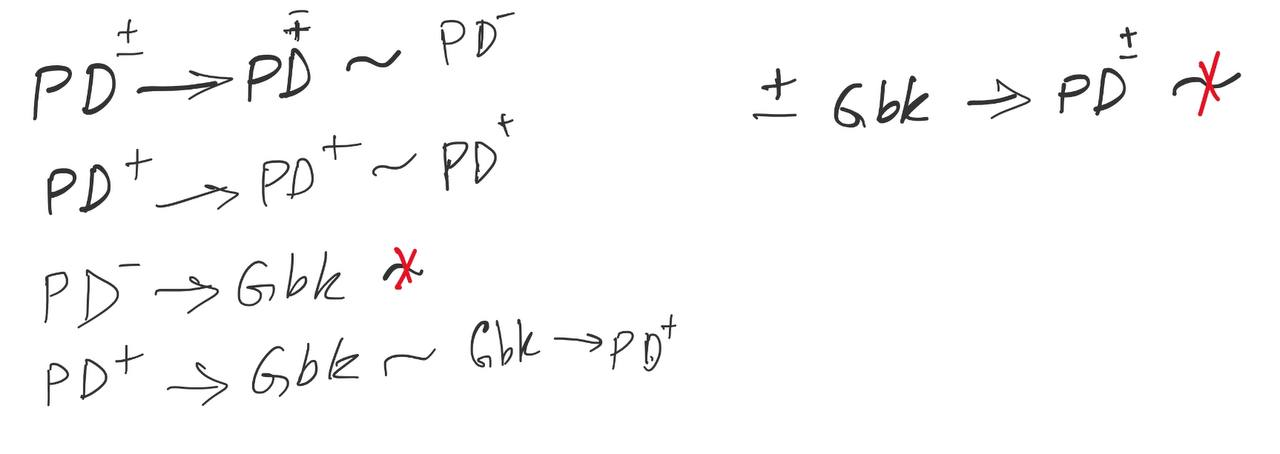
\includegraphics[width=0.7\textwidth]{img/rule1.jpeg}
    \caption{Правила roren $\xrightarrow{}$ roren}
    \label{fig:rule1}
\end{figure}

\begin{algo}
Сначала перестроим граф $G$ по правилу $F \xrightarrow{} \$Transform* \sim \$Transform$, где $Transform$ - это некоторое преобразование, которое после перестройки может иметь несколько входов (рис.~\ref{fig:flatten}).\\
\begin{figure}[h]
    \centering
    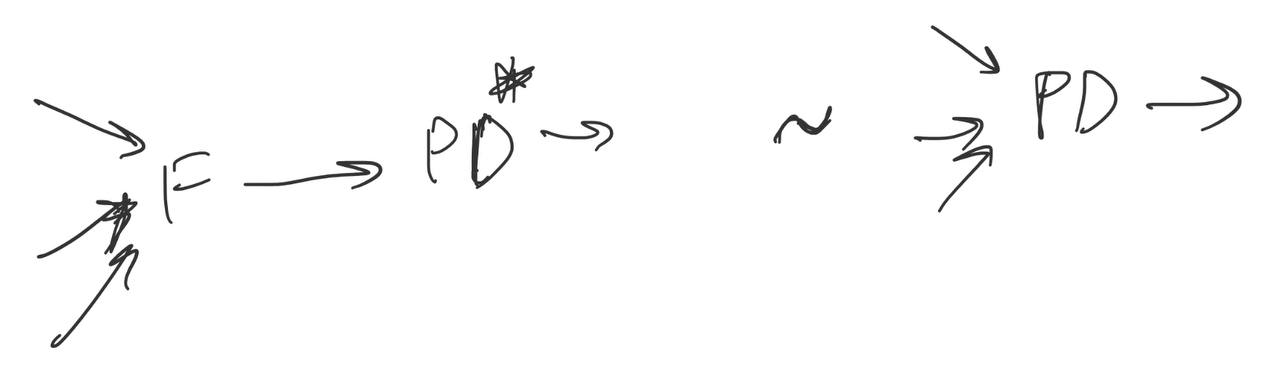
\includegraphics[width=0.5\textwidth]{img/flatten.jpeg}
    \caption{Преобразование с Flatten}
    \label{fig:flatten}
\end{figure}

Построим слоистую сеть $R$ по $G$ (рис.~\ref{fig:net}).\\
\begin{figure}[h]
    \centering
    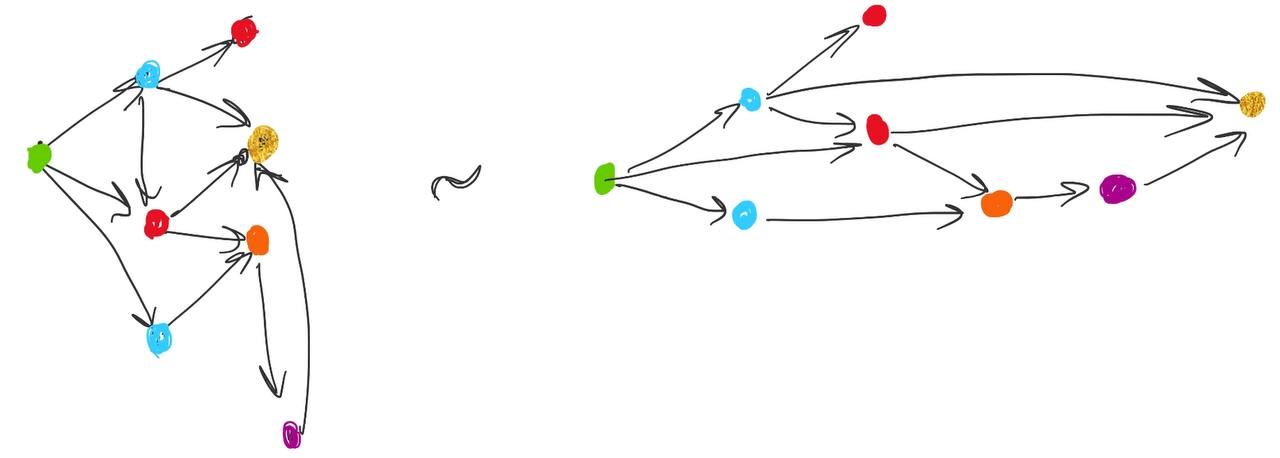
\includegraphics[width=0.8\textwidth]{img/net.jpeg}
    \caption{Построение слоистой сети}
    \label{fig:net}
\end{figure}

Теперь будем проходить по $R$. Шаг обхода будет состоять из двух стадий: collapse и expand. На стадии collapse некоторые вершины сливаются, на стадии expand новые вершины добавляются в рассмотрение. Обход будем делать по слоям, рассматривая текущий и следующий, по ходу присваивая вершинам цвета:\\
\begin{itemize}
    \item черные - ещё не посещенные вершины, на слоях отличных от текущего и следующего,
    \item оранжевые - посещенные вершины, на текущем слое или на предыдущих слоях, если есть ребро в черную вершину,
    \item красные - не посещенные вершины, находящиеся на следующем слое,
    \item зеленые - посещенные вершины, которые больше не будут участвовать в слиянии.
\end{itemize}
При старте обхода помечаем первый слой оранжевым цветом, второй слой красным.\\
На произвольном шаге алгоритма рассматриваем каждую из оранжевых вершин отдельно. Сначала идет стадия collapse. На данном этапе может возникнуть 2 типа коллизий (рис.~\ref{fig:collision}), которые можно пытаться разрешать через pattern-matching или оставлять как есть\\
\begin{figure}[h]
    \centering
    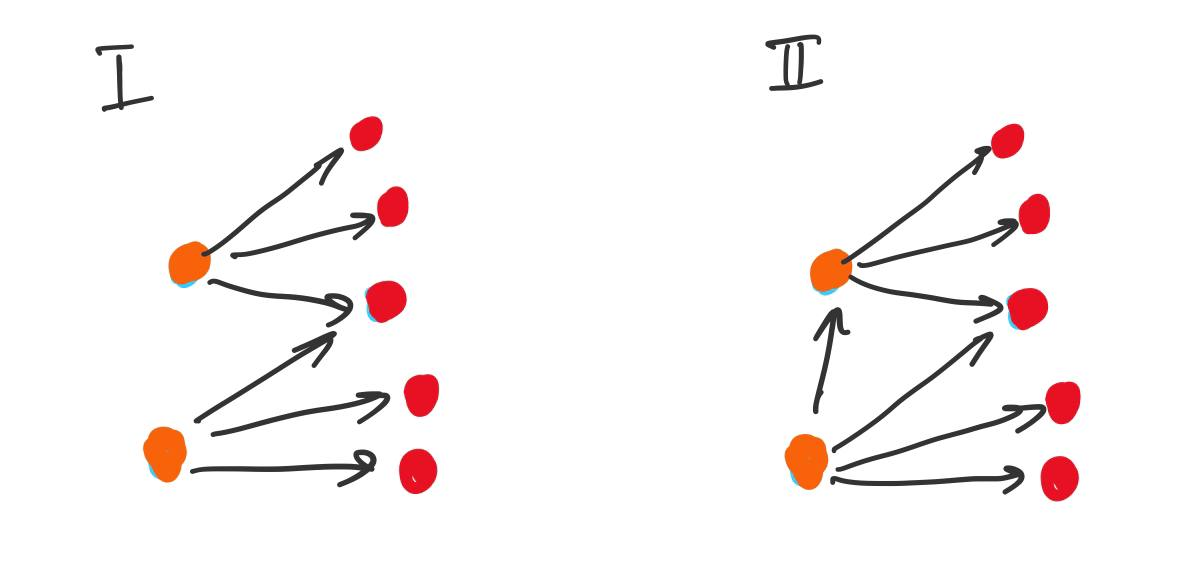
\includegraphics[width=0.7\textwidth]{img/collision.jpeg}
    \caption{Типы коллизий}
    \label{fig:collision}
\end{figure}

Для вершин, в которых не возникает коллизий, применяя правила roren $\xrightarrow{}$ roren, можно влить красную вершину в оранжевую.\\
После начинается стадия expand, оставшиеся красные вершины окрашиваются в оранжевый, текущий слой продвигается вперед. Сейчас оранжевые вершины с прошлого слоя могут стать зелеными, в случае если все ребра входят в оранжевые вершины.\\
Пример обхода приведен на рис.~\ref{fig:algo}.\\
\begin{figure}[h]
    \centering
    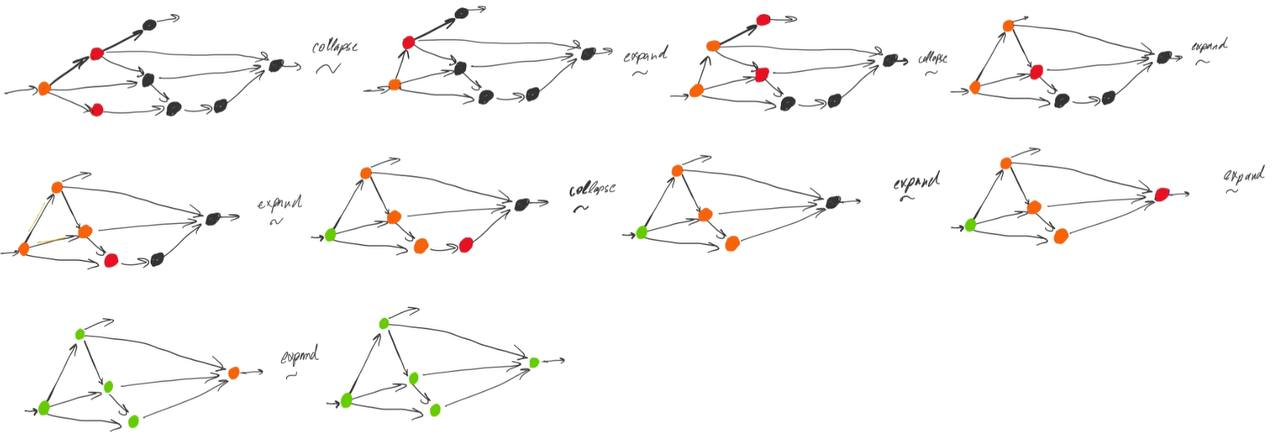
\includegraphics[width=\textwidth]{img/algo.jpeg}
    \caption{Пример обхода}
    \label{fig:algo}
\end{figure}

После того, как завершился обход по сети $R$. Можно перевести граф в операции Map, Reduce и MapReduce по правилам roren $\xrightarrow{}$ YT (рис.~\ref{fig:rule2}).\\
\end{algo}

\begin{figure}[h]
    \centering
    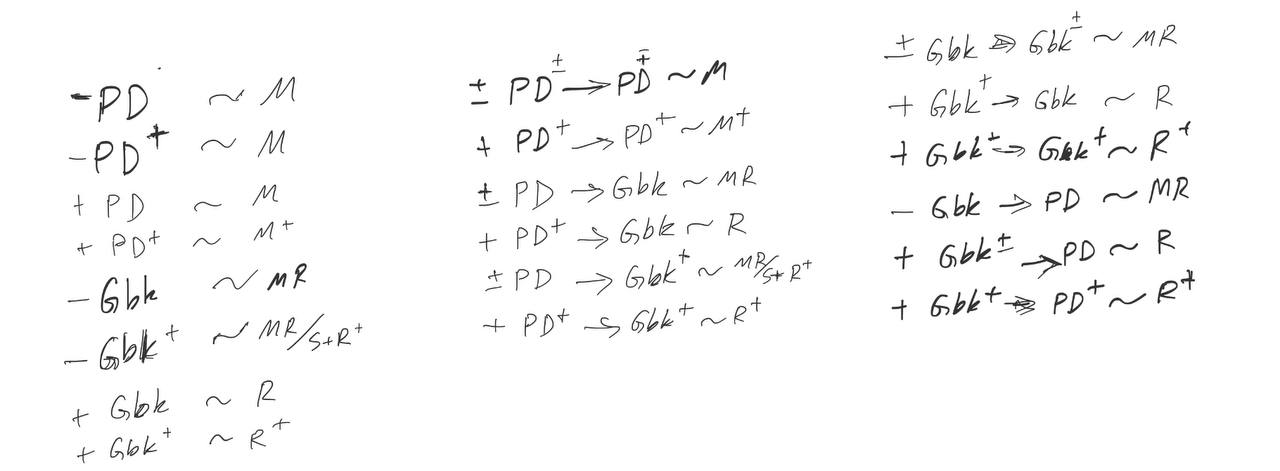
\includegraphics[width=\textwidth]{img/rule2.jpeg}
    \caption{Правила roren $\xrightarrow{}$ YT}
    \label{fig:rule2}
\end{figure}

На самом деле, в алгоритме есть несколько точек кастомизации поведения.\\
\begin{itemize}
\item Мы можем пытаться разрешать коллизии (рис.~\ref{fig:collision}) первого типа без pattern-matching-a - сливать две оранжевые вершины
\item После преобразований размер данных по ключу может сильно меняться: уменьшаться, если трансформ фильтрует данные, увеличиваться, если дробит
\item Можно сливать независимые ветки графа, но стоит думать об отсутствии параллельности исполнения в данном случае
\item У операций в качестве атрибутов могут быть выставлены лимиты на ресурсы, которые есть возможность учитывать при слияниях
\item Прежде чем применять во всех местах правила слияния с учетом сортированности, можно сделать предпроход и понять до каких входом прокидывается сортированность
\item Combine распадается в два Reduce; Flatten, после которого не шло никаких Transform, станет YT Map-ом
\item Если у Transform-а есть side выход и ребро в другой Transform, то можно не делать временную таблицу
\end{itemize}



\newpage
\subsection{Оптимизатор}

Стадия оптимизации подразумевает несколько обходов по заранее построенному RorenGraph-у.

\subsubsection{Стратегии оптимизации}

В оптимизаторе отдельно выделен интерфейс IStrategy (рис~\ref{fig:strat}), позволяющий коллапсировать оранжевую и красную вершину связанные ребром. Важно, что этот случай подразумевает, что нет другой оранжевой вершины, ребра которой ведут в рассматриваемую красную.

\begin{figure}[h]
    \centering
    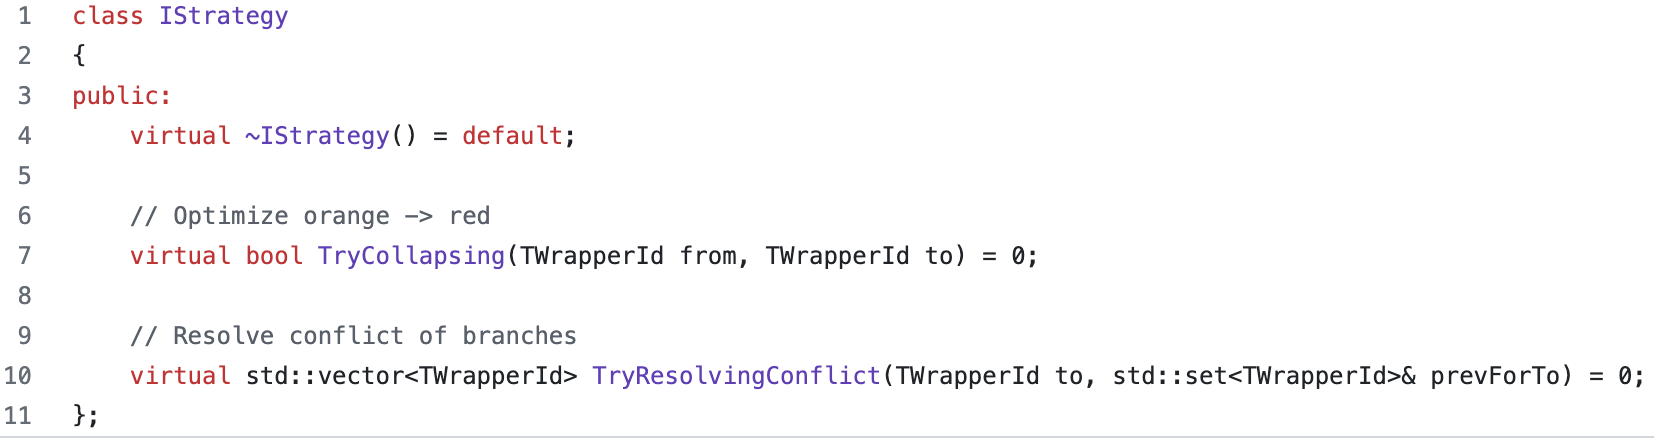
\includegraphics[width=\textwidth]{img/strat.png}
    \caption{Интерфейс стратегии конденсации вершин}
    \label{fig:strat}
\end{figure}

Помимо этого IStrategy позволяет разрешить конфликтную ситуацию, когда есть множество оранжевых вершин, ребра которых ведут в общую красную вершину.

Реализацией данной стратегии может быть стратегия, которая коллапсирует вершины и разрешает конфликты.

Однако это далеко не единственный вариант. Пользователям может понадобится стратегия, которая не сливает параллельные ветви, т.к. это увеличивает latency готовности конкретных таблиц.

Также пользователи могут иметь вычислительно тяжелые операции, требующие большого количества RAM. Так, в случае отдельного запуска операций проблем не будет, но при их слиянии памяти, отведенной на один job, может не хватить.

\newpage
\subsubsection{Предобход для Flatten}

В дизайн Roren заложена концепция, которая позволяет легко описывать в коде графы. Она состоит в том, что у transform-а может быть только один вход. В случае графов с Flatten такой дизайн приведет к тому, что требуется рассматривать несколько слоев transform-ов. Также для упрощения алгоритма мы рассматриваем граф, состоящий из transform-ов, не обращая внимания на коллекции, но сохраняя их.

Для того, чтобы перейти к упрощенному графу требуется сделать предобход, который удалить из графа Flatten, соединяя предыдущие и последующие transform-ы напрямую.

\newpage
\subsection{Дополнения алгоритма}

\subsubsection{Сохранение сортированности}

\newpage
\subsubsection{Когда не стоит оптимизировать}

